\newcommand{\mypathjcc}{../thesis/jcc}
\newcommand{\mypathjccdata}{../thesis/jcc/data}
\newcommand{\bE}{\mathbb{E}}
\newcommand{\E}[2]{\mathbb{E}_{#1} \left[ #2 \right]}
\newcommand{\bP}[2]{\mathbb{P}_{#1} \left[ #2 \right]}
\newcommand{\dpO}{d\mathbb{P}_\Omega}
\newcommand{\feb}{f_e\left(\beta\right)}
\newcommand{\fenb}{f_{en}\left(\beta\right)}
\newcommand{\fehb}{f_e\left(\hat{\beta}\right)}
\newcommand{\pfeb}{\frac{\partial}{\partial \beta_j}\feb}
\newcommand{\pfenb}{\frac{\partial f_{en}\left(\beta \right)}{\partial \beta_j}}
\newcommand{\pfehb}{\frac{\partial f_e\left(\hat{\beta} \right)}{\partial \beta_j}}
\newcommand{\hye}{\hat{y}_e}
\newcommand{\hse}{\hat{s}_e}
\newcommand{\pe}{\pi_e}
\newcommand{\pn}{\pi_n}
\newcommand{\psen}{\psi_{en}}
\newcommand{\rand}{\boldsymbol{\delta}}
\newcommand{\ri}{\pmb{\delta^m}}
\newcommand{\rf}{\pmb{\delta^y}}
\newcommand{\rx}{\pmb{x}}
\newcommand{\rD}{\pmb{\Delta}}
\newcommand{\rdm}{\pmb{\delta^m}}
\newcommand{\rdmk}{\pmb{\delta^m_k}}
\newcommand{\rdy}{\pmb{\delta^y}}
\newcommand{\hry}{\pmb{y}}
\newcommand{\hy}{y}
\newcommand{\rz}{\pmb{z}}
\newcommand{\sD}{\sigma_\Delta^2}
\newcommand{\se}{\sigma_e^2}
\newcommand{\sn}{\sigma_n^2}
\newcommand{\sen}{\sigma_{en}^2}
\newcommand{\see}{\sigma_{ee}^2}
\newcommand{\sko}{\sum_{k_1}}
\newcommand{\skt}{\sum_{k_2}}
\newcommand{\sigot}{\Sigma_{k_1,k_2}}
\newcommand{\irzp}{\E{\Omega}{g(\hry_e)}}
%\newcommand{\rw}{{w(\omega)}} %\newcommand{\rx}{{x(\omega)}} %\newcommand{\ry}{{y(\omega)}}
\newcommand{\Ery}{\E{\Omega}{\ry}}
\newcommand{\Erx}{\E{\Omega}{\rx}}
\newcommand{\Erdm}{\E{\Omega}{\rdm}}
\newcommand{\ErD}{\E{\Omega}{\rD}}
\newcommand{\tB}{\tilde{B}}
\newcommand{\tx}{\tilde{x}}
\newcommand{\ttheta}{\tilde{\theta}}

\chapter{Line~Failure~Risk~Models for Real-Time Dispatch}\label{jcc-chapter}

\section{Introduction}

The use of optimization models for operation of bulk power systems has been critical in creating efficient markets for wholesale power generation over the last few decades.  Optimization models are solved to clear multiple markets, including day ahead and real time markets, while maintaining physical constraints related to generator characteristics and power flow constraints on the high voltage transmission system. The nonlinear and nonconvex equations for balanced three phase power flow make these problems particularly difficult to solve and approximations, such as decoupled (DC) power flow, are commonly used in economic models. 
%The full nonlinear models are seen in reliability focused problems and design problems such as capacitor placement and can solved via local methods or convex relaxations \cite{hijazi_2015,lavaei_2012}.  
These optimization models and solution methodologies have become standard tools for independent system operators tasked with operating the bulk power system.

In this chapter, we focus on the operation of the real time dispatch market (five minutes and less) and the associated reliability issues.  Reliability issues have a large impact on the economy, estimated at \$79 billion in 2001 \cite{lacommare_2006}, relative to the total cost of electricity, \$247 billion in 2001 \cite{eia_gov}.  Additionally, large power outages are disruptive to society, are costly (the 2003 Northeast blackout was an estimated loss of \$6.4 billion to the economy), and can lead to the loss of life \cite{northeast_2003}.  Blackout frequency changes seasonally and with the time of day.  The load shed from blackout events follows a power-law distribution where large blackout are more likely than expected \cite{hines_2009}.  This blackout distribution has been stable over the last thirty years and represents a dynamic equilibrium \cite{dobson_2007,hines_2009}.  Small frequent blackouts are associated with small reserve margins in generation and large infrequent blackouts are associated with a highly utilized transmission system \cite{dobson_2007}.  We develop a risk measure that captures the utilization of transmission elements in a systems perspective.  This is similar to the use of severity measures to capture line loading risks from a systems perspective \cite{vrakopoulou_2013c,wang_2014,wang_2013}.  Our model is equivalent to their system risk measure when there is fixed demand and we use a linear approximation of the risk measure.  However, we solve our original log-convex risk measure exactly via nonlinear programming. We also extend our model to the case of a multivariate Gaussian distribution for net injection uncertainty where we make a linear approximation to retain a tractability.

There has been increased importance placed on models that account for the growing generation uncertainty due to renewables such as wind and solar.  This uncertainty is being  handled for the traditional line threshold model of economic dispatch using chance constraints (CC).  Several groups have developed chance constrained models to ensure that the power flow on any transmission element is less than its capacity for a large percentage of scenarios.  Several extensions are made which involve arbitrary slack distribution \cite{bienstock_2012}, application to large penetration of wind farms \cite{vrakopoulou_2013b}, with HVDC lines \cite{vrakopoulou_2013}, and others \cite{roald_2013,vrakopoulou_2013c} which is discussed in \Cref{chanceconstraints}.  Instead of relying on the traditional line threshold, we directly enforce a constraint on the quantity of interest, the probability that a line will fail. The nominal capacity of transmission elements is based on thermal characteristics of the line as well as a set of environmental characteristics, which represent the worst case scenario for different operating times.  Typically, there may be a summer rating and a winter rating for each transmission element, where the winter rating has colder ambient temperature (less heating and less sagging) thus a higher capacity.  The limiting constraint determining the line capacities are typically due to the acceptable sagging level derived from a predetermined risk level of fault \cite{seppa_2007}.  Dynamic line limits are being explored to account for real time environmental conditions \cite{bucher_2013,wang_2011,yip_2009,zhang_2002}.  

In this chapter, we quantify the endogenous risk of line failure due to line loading.  Exogenous failure events, primarily caused by weather, such as falling tree limbs taking out circuits, are accounted for through the N-1 security requirements.  In order to quantify the endogenous risk, we make several assumptions on the failure density function, which are used elsewhere in literature and have a physical interpretation.  Our failure density function assumes that below some loading level there is no endogenous risk associated with the loading and that above a critical level the risk is monotonically increasing.  We use a piecewise linear function to model the risk and this model has been used in cascading power failure research in papers \cite{carreras_2002,chen_2005,dobson_2007,hines_2011,newman_2011}.  While there is a hard limit on transmission lines that causes them to trip with certainty (due to protective relay elements), the system is always operated far away from these points.  If the system was operating close, random fluctuation in power injects would cause the system to trip much more regularly than is seen.  Our model is built on the assumption that increasing power flow increases the risk of line failure, and we can only make probabilistic statements about these failure rates. 


We combine individual line risks to form a system risk measure that represents the probability that one or more lines fail (due to loading), which we constrain to be small depending on the operators' risk tolerance.  The combination of a system risk measure and demand uncertainty leads to our joint chance constraint (JCC) model.  When there is no uncertainty in demand and generation, this  system can be solved exactly using nonlinear programming and its linear approximation reduces to other system risk models that have apeared in literature \cite{vrakopoulou_2013c,wang_2013}.  Under demand uncertainty, the line risk's failure becomes dependent on both the mean and standard deviation of line flow. In order to solve this model, a linearization of the system risk measure is made.  Once this approximation is made, the problem becomes solvable for large test instances even when exogenous N-1 contingencies are considered.  
%%
In section \Cref{economicdispatch} we look at the standard economic dispatch model, referred throughout as optimal power flow (OPF).  Using the DC power flow approximation, we show the linear program used in the real time market with a quadratic cost function. In the following \Cref{chanceconstraints}, we begin by exploring the uncertainty introduced into the system by wind generation and variable load.  We then show the chance constraints (CC) used in other work to ensure the reliability constraints are met a large percentage of the time.  In \Cref{jointchanceconstraint}, we develop a system risk measure defined by the probability that one or more lines fail by assuming the probability a line fails is related to line loading and can be represented by a piecewise linear function.  Using this risk measure and the assumption of fixed generation and demand, we can solve this model exactly using nonlinear programming.  Finally, we look to combine uncertain wind and load with our system risk measure.  Under the assumption of a multivariate Gaussian distribution for wind and load, we find the covariance matrix to enforce the resulting variation in branch flows.  The risk constraints are convex with respect to the mean and standard deviation of branch flow.  We then describe the solution methodology in  \Cref{solutionmethodology} which uses an iterative algorithm and cutting planes to describe the convex risk constraints.  Finally, we explore the computational results in \Cref{computationalresults} to understand the characteristics of the standard economic dispatch model, chance constraint model, and our joint chance constraint model.


In order to solve our problem, a cutting plane algorithm is used to underestimate the line risk function (convex, not analytic) as well as the branch flow standard deviations (second order cone).  This multiobjective problem of cost and risk form a frontier that is shown in the computational section.  The OPF and CC models give dispatch points on the interior of this frontier, which are inefficient according to our system risk measure.  The CC and JCC models take around the same amount of time to solve and are an order of magnitude slower than OPF.  Our JCC model can reduce the expected number of lines over their hard threshold compared to the CC model, which is what the chance constraint model aims to do on an individual line level.  Finally, our JCC model is robust to deviations in line risk parameters as well as other failure density function models. 




%%%%%%%%%%%%%%%%%%%Section 2, DC dispatch introduction
\section{Economic Dispatch Models}\label{economicdispatch}
Bulk power systems rely on dispatch models to clear the markets for power in a timely manner.  These models are critical to ensure that the market is cleared minimizing cost while maintaining a set of reliability constraints. The DC power flow model is typically used to clear economic markets for both real-time and day-ahead operation, where the day-ahead operation has the additional complexity of committing slow ramping resources and is solved with mixed-integer programming. 


\subsection{Optimal Power Flow using DC approximation} 
The DC power flow model is a simplification of the AC power flow model, which more accurately represents the true physics of the balanced three phase electrical system.  The DC model makes the assumptions that the power lines are lossless, voltages are equal to nominal, and the phase angle differences are small.  While losing some accuracy and important information about the voltages, the problem becomes more tractable.  Methods can be used to find approximate voltages, which can be important indicators for system stability.  Additional complexities are  ignored for clarity such as shunt elements which consume power \cite{matpower}.

The topology of the power grid, with $N_l$ lines and $N_b$ buses, can be represented using an incidence matrix, $C \in \R{N_l \times N_b}$, where $c_{ei}=1$ if line $e$ begins at node $i$ and $-1$ if line $e$ ends at node $i$.  The set of all edges is denoted as $\cE$ and the set of all nodes as $\cI$.  In the DC power flow model, the line susceptance is the constant of proportionaility between bus voltage and liv, so let $D=diag\left(b_1,b_2,...b_{N_l}\right)$ be the diagonal susceptance matrix.  The branch flows $y \in \R{N_l}$ for given a set of phase angles $\theta \in \R{N_b}$ at each bus are determined by Kirchoff's Current Law and can be written as
\begin{equation}\label{kcl}
y=D C \theta
\end{equation}
for the DC power flow model.  This results in the typical DC line constraints $y_{e} = b_{e} (\theta_i - \theta_j)$ for each line $e$ connecting from node $i$ to node $j$.  Applying $C^T$ to the branch flows $y$ in \Cref{kcl} give the net injects for a given set of branch flows and represents conservation of energy at each node.
  The system matrix $B = C^T D C$ can be used to write the DC power flow equations for the net injects $x \in \R{N_b}$
\begin{equation}\label{dcpow}
x = C^T y = B \theta
\end{equation}
This equation has one degree of freedom and by removing the slack bus inject (row) and phase angle (column), then the following system
\begin{equation}
\tx = \tB \ttheta
\end{equation}
has a unique solution.   Here, $\tx \in \R{N_b-1}$ has the slack node removed and $\tilde{B}$ is a $(N_b-1) \times (N_b-1)$ matrix with the row for the slack bus inject and the column for the slack bus angle has been removed.  The OPF model uses the DC simplifications from the full AC model to ensure the model can be solved reliably in a timely manner.  A standard OPF model is shown here and used in the computational section.

The following program \Cref{opf_program} is minimizing a quadratic cost function of generation $x_j$ for each generator $j$ in the set of all generators $\cJ$ with cost coefficients $c^2_j, c^1_j$ and $c^0_j$.  There are two incidence matricies, $c_{ij}^g$ for generators and $c_{ie}^b$ for branches.  $c_{ij}^g$ takes the value 1 when generator $j$ is connected to node $i$ in the set of all nodes $\cI$.  $c_{ie}^b$ takes the value 1 if the edge $e$, in the set of all edges $\cE$, originates in node $i$ and a -1 if edge $e$ terminates in node $i$.  We also have nominal demand $d_i$ for each node $i$, branch capacities $U_e$ for each branch $e$, and generator limits $G^{min}_j$ and $G^{max}_j$.
\begin{subequations}
\label{opf_program}
\begin{alignat}{3}
\textbf{OPF:= }\min_{\left(x;\theta,y\right)} && \multispan{2}{$\displaystyle\sum_{j \in \cJ} \left[  c^2_j x_j^2 + c_j^1 x_j + c_j^0 \right]$}  & \label{jcc_obj}\\
%\min_{\left(x,\beta,;\theta,y\right)} && \multispan{2}{$\displaystyle\sum_j \left[  c_2 \left(x_j^2 + \beta_j^2 \sD \right) + c_1 x_j + c_0 \right]$}  & \label{jcc_obj}\\
                        &&  \sum_{j \in \cJ} c^g_{ij} x_j - \sum_{j \in \cJ} c^b_{ie} y_e          &=d_i       && \forall i \in \cI \label{opf_cons}\\ 
                 && y_e - b_e \sum_{i \in \cI} c^b_{ie} \theta_i          &=0         && \forall e \in \cE \label{opf_kcl}\\
                 && y_e &\in \left[ -U_e, U_e \right] && \forall e \in \cE  \label{opf_limit}\\
                 && x_j &\in \left[ G^{min}_j, G^{max}_j \right] && \forall j  \in \cJ \label{opf_gen}  
\end{alignat}
\end{subequations}


\section{Chance Constraints for Random Branch Flows}\label{chanceconstraints}



As the penetration of renewables increases, there is an increasing interest in the inclusion of uncertainty in dispatch models.  The primary approach has been to treat wind generation and load variables as random variables and enforce probabilistic constraints replacing the standard deterministic reliability constraints.  Probabilistic constraints, or chance constraints, enforce that a constraint involving a random variable must be satisfied a large percentage of the time.  Chance constraints have been used in a variety of power system problems, from a unified model including large wind penetration and HVDC lines \cite{vrakopoulou_2013c}, to models using an arbitrary slack distribution \cite{bienstock_2012}.  Additionally, their are models that have different assumptions on the probability distributions of the random variables, from the common independent Gaussian assumption \cite{bienstock_2012,roald_2013} to no assumption on the uncertainty except for the ability to sample from it \cite{vrakopoulou_2013,vrakopoulou_2013c,vrakopoulou_2013b}.



We look first at chance constraints for branch flows, which begins by looking at the root uncertainty in net injections due to wind and load. The deviation of net injections from forecast leads to a response by automatic generator control to ensure that supply and demand are constantly in balance.  Under the DC power flow model, the branch sensitivities to changes in net injections are a linear relationship.  This allows us to calculate the uncertainty in branch flows dependent on the uncertainty in wind and load.  A common assumption is that the uncertainty in deviation from forecast is a Gaussian distribution,  and that its mean and covariance is known.  This assumption allows for a tractable formulation of the chance constraint without sampling from the uncertainty distribution. 

\subsection{Random Power Flows}
The power injections at each node are subject to random fluctuation over varying time intervals.  The variation over the 5 minute time scale are dealt with using ancillary services such as regulation and reserve.  The sources of the fluctuations can be due to random demand or generation.  These fluctuations affect the power flows on transmission lines and cause a linear shift in the approximated DC power flow model.  The risk of the system is dependent on the characteristics of these resulting random power flows.  In greater time intervals, the generators can redispatch for economic or reliability reasons.


Over the course of the 5 minute interval dispatch period, demand  fluctuates from its expectation.  This  fluctuation can be due to the behaviors of aggregated residential load, commercial or industrial processes, or power production for renewable sources such as wind and solar.  Assuming these random injects are Gaussian, the linear approximations made in the DC power flow leads to the branch flows also being Gaussian random variables.  The mean vector and covariance matrix of branch flows can be calculated if the mean and covariance of the random injections are known.

Let $\ri \in \R{N_m}$ be a random vector describing the deviation from forecast on a subset of nodes $k \in \cM$ which are random ($| \cM | = N_m$).  Bold lettering $\ri$ represents a random variable with a probability distribution supported on $\bD$.  Define an incidence matrix $C_M \in \R{N_b \times N_m}$ where $c_{im}=1$ if random inject $m$ is connected to node $i$.  Additionally, we define the forecasted demand at each node as $d \in \R{N_b}$ where $N_b$ is the number of buses.  The forecasted demand is supplied by generation $x^g \in \R{N_g}$ where $N_g$ is the number of generators and the incidence matrix $C_g$ brings them into the bus space.    The vector of net injections are defined by 
\begin{equation}\label{rand_inj}
 \rx = C_g\left(x^g+\beta \rD\right) - (d + C_M \ri) 
\end{equation}
 where the left term is generation/controllable and the right term is load/uncontrolled.  Both terms have a fixed component due to the forecasted system and a random component due to the random injections.  For the rest of this chapter, we assume the random injects $\ri$ are assumed to be a multivariate Gaussian distribution with known mean $\mu^m$ and covariance $\Sigma^m$.  

The random injects cause loading on the transmission lines to fluctuate and the flows are random variables themselves. Taking the derivative of \Cref{dcpow}, we get $d \tx = \tilde{B} d \ttheta $.  The changes to the phase angles given a vector of changes to net injects is $ d \ttheta = \tilde{B}^{-1} d \tx $.  This can be used to find the sensitivity of branch flows to net injects 
\begin{equation}\label{isf}
 d y = A d x 
\end{equation}
where $A$ is the injection shift factor matrix $A = D C \left[\begin{array}{cc} 0 & \tilde{B}^{-1} \end{array} \right]$ and $0\in \R{N_b}$ is a column of zeros.  For a slack distribution $\beta$ with $\sum_{j \in \cJ} \beta_j=1$ and aggregate demand change $\Delta = \sum_{i \in \cI} dx_i$, the net injects also change by $- \beta \Delta$ so that $dy = A\left( dx - C_g \beta \Delta \right)$.  The random power flows $\ry$ can be found by applying \Cref{kcl,dcpow} to the random net injections \Cref{rand_inj}
\begin{equation}\label{rand_flow}
 \ry = y^0+ A C_G \beta \rD  - A C_M \rdm 
\end{equation}
with 
\begin{equation}
\rf = A C_G \beta \rD - AC_M \ri
\end{equation}
being the random component of branch flows.
Without loss of generality, we can assume that the random injects have zero mean.  If we know them to have a nonzero mean, we can shift the forecasted system to account for it. 
The forecasted system  $\left(x^g, y^0, \theta^0\right)$ is the expectation of \Cref{rand_inj,rand_flow}
\begin{align*}
C_G x^g - d &= C^T y^0 \\
y^0 &= B^T C \theta^0 
\end{align*}
with zero mean $\Erdm=\left[0 \cdots 0\right]^T$ and $\ErD=0$. 
From \Cref{isf}, we have that the random component of the flow is made part from the random injects and part the generators response.   The random branch flows $\rf$ are a linear function of the random injects $\ri$, thus $\ry$ has a multivariate Gaussian distribution as well.  The branch covariance matrix can be calculated
\begin{equation*}
\E{\bD}{ \left( \ry - \mu^y \right) \left( \ry - \mu^y \right)^T } = \E{\bD}{\left( A(C_G\beta \vec{1}^T - C_M) \ri \right) \left( A(C_G\beta \vec{1}^T - C_M )\rdm \right)^T } 
\end{equation*}
where $\vec{1} = \left\{ 1 \right\}^{N_m}$ is a vector of ones that is of $N_m$ length.  Substituting $G=A(C_G\beta \vec{1}^T - C_M)$, we have
\begin{align*}
 \E{\bD}{\left( G \ri \right) \left( G \rdm \right)^T } &=  \E{\bD}{ G  \ri \rdm^T G^T } \\
 &= G  \E{\bD}{ \ri \rdm^T } G^T 
\end{align*}
Since the expectation is linear and the covariance $\Sigma^m$ of $\ri$ is known ($\Sigma^m = \E{\bD}{\ri \ri^T}$), we have power flow covariance matrix, after substitution of $G$, of
\begin{equation}\label{branch_cov}
\Sigma^y = A(C_G\beta \vec{1}^T - C_M) \Sigma^m (C_G\beta \vec{1}^T - C_M)^T A^T.
\end{equation}

This equation can be found piecewise by taking the variance of the random component of the branch flow for a given branch $e$ and substituting $\pi_e = \sum_{j \in \cJ} A_{ej} \beta_j$ (the effect on branch $e$ from aggregate deviation from forecast $\Delta$).  Reforming this assumption, we have the random component of branch flow $\rdfe$ on branch $e$ defined by
\begin{align*}
  \rdfe &= \sum_{j \in \cJ} A_{ej} \beta_j \rD - \sum_{k \in \cM} A_{ek} \rik\\
&= \pi_e \sum_{k \in \cM} \rik - \sum_{k \in \cM} A_{ek} \rik\\
&= \sum_{k \in \cM} \left[ \pi_e  - A_{ek} \right] \rik 
\end{align*}
where $\rik$ is the random inject $k \in \cM$. Using the notation that the covariance between random inject $k_1$ and $k_2$ is $\Sigma_{k_1 k_2} = \operatorname{CoVar}[ \rikk ,\rikkk ]$, the covariance between branch $e_1$ and $e_2$ is calculated by
\begin{subequations}\label{covar_branch}
\begin{align}
\operatorname{CoVar}[ \rdfee,\rdfeee ] &=  \sum_{k_1 \in \cM} \sum_{k_2 \in \cM} (\pi_{e_1} - A_{e_1 k_1}) (\pi_{e_2} - A_{e_2 k_2}) \Sigma_{k_1 k_2} \\
\operatorname{CoVar}[ \rdfee,\rdfeee ] &=  \pi_{e_1} \pi_{e_2} \sum_{k_1 \in \cM} \sum_{k_2 \in \cM} \Sigma_{k_1 k_2} \\
& -  \pi_{e_1} \sum_{k_1 \in \cM} \sum_{k_2 \in \cM} A_{e_2 k_1} \Sigma_{k_1 k_2} - \pi_{e_2} \sum_{k_1 \in \cM} \sum_{k_2 \in \cM} A_{e_1 k_1} \Sigma_{k_1 k_2}   \\
&+ \sum_{k_1 \in \cM} \sum_{k_2 \in \cM} A_{e_1 k_1} A_{e_2 k_2} \Sigma_{k_1 k_2}  \\
\operatorname{CoVar}[ \rdfee,\rdfeee ] &=  \pi_{e_1} \pi_{e_2} \sD -  \pi_{e_1} \setwo - \pi_{e_2} \seone   + \seealone
\end{align}
\end{subequations}
where  $\sD, \se,$ and $\seealone$ are all pre-computable parameters given by the following equations
\begin{subequations}
\begin{align}
 \sD &= \sko \skt \sigot  \\
 \sigma^2_e &= \sko \skt A_{ek_1} \sigot   \hspace{15px} \forall e \in \cE\\
 \seealone &= \sko \skt A_{e_1 k_1} A_{e_2 k_2} \sigot \hspace{15px} \forall e_1,e_2 \in \cE.
\end{align}
\end{subequations}



There are two primary parts to the variance in line flow, that from the uncertain random injects and that from the aggregate deviation from forecast at the slack distributions response.  The variance of branch flow on line $e$ is described as follows  
\begin{equation}
\operatorname{Var}[ \rdfe ] =  \pi_e^2  \sD  - 2 \pi_e \sigma^2_e  + \sigma^2_{e e}  \hspace{15px} \forall e \in \cE
\end{equation}



When the net injections are uncertain, the branch flows are also uncertain and represented by $\ry_e$ for branch $e$, where the bold letter denotes a random variable throughout this chapter.  Let $\epsilon_l$ be the percentage of time we allow the constraint to be violated for each line $l$, so that the following constraint 
\begin{equation}\label{eq_cc}
 \bP{\Omega}{  -U_ \leq  \ry_e \leq U } \geq 1- \epsilon_l \hspace{10px} \forall e \in \cE
\end{equation}
represents the chance constraint version of the nominal line capacity limit.  Assuming $\ry_e$ is a Gaussian random variable with mean $\mu^y_e$ and standard deviation $\sigma^y_e$. Given a line risk preference $\epsilon_l$, we have 
\begin{equation}\label{etaequation}
\eta_l = \Phi^{-1}\left(1-\epsilon_l\right)
\end{equation}
 where $\Phi^{-1} ( \cdot )$ is the inverse of the standard normal distribution. The following constraints
\begin{align*}
 \mu^y_e + \eta_l \sigma^y_e \leq U_e  \hspace{10px} \forall e \in \cE \\
 \mu^y_e - \eta_l \sigma^y_e \geq -U_e  \hspace{10px} \forall e \in \cE
\end{align*}
are deterministic constraints for \Cref{eq_cc}

In addition to chance constraints on branch flows, the output of generators may be uncertain.  Let $\rD$ represent the aggregate deviation from forecast that the generators must respond to.   The slack distribution is a subset of generators who are able to respond to deviations in forecast in a fast time scale.  They typically follow a signal such as the area control error (ACE).  Let $\beta_j$ define this slack distribution, where $\beta_j$ is the portion of $\rD$ that generator $j$ compensates for.  We know that $\sum_{j \in \cJ} \beta_j =1$ for demand to be satisfied exactly.  Additional constraints can be put on the slack variables $\beta$ depending on generator characteristics and their ability to respond to variations in load.  The total output for generator $j$ is $x_j + \beta_j \rD $
and we enforce its constraints probabilistically since it is a random variable.  Assuming that the individual variations in wind and load are Gaussian, their aggregate is also Gaussian.   Let $\epsilon_j$ be the probability that the constraint can be violated for generator $j$ and we would like a constraint to enforce
\begin{equation}\label{eq_cc_gen}
\bP{\Omega}{ G^{min}_e \leq x_j + \beta_j \rD  \leq G^{max}_e } \geq 1 - \epsilon_j \hspace{10px} \forall j \in \cJ 
\end{equation}
where $G^{min}_e, G^{max}_e$ represent the minimum and maximum output of the generator over the given time interval and accounts for ramping constraints and already made commitment decisions. Since $\E{\Omega}{\rD} = 0$ and the standard deviation of $\rD$ is known, which takes the value $\sigma_\Delta$, the following constraints to enforce \Cref{eq_cc_gen} are
\begin{align*}
x_j + \beta_j \sigma_\Delta \eta_g &\leq G^{max}_j \hspace{10px} \forall j \in \cJ \\
x_j - \beta_j \sigma_\Delta \eta_g &\geq G^{min}_j \hspace{10px} \forall j \in \cJ .
\end{align*}

By allowing the slack distribution to be variables in the optimization procedure, the cost to meet load is now a random variable.  Assuming we would like to minimize the expected cost of generation, we would like to minimize
\begin{equation*}
\E{\Omega}{ \sum_{j \in \cJ} \left[ c^j_2 (x_j+\beta_j \rD)^2 + c^j_1 (x_j + \beta_j \rD) + c_0^j \right] }
\end{equation*}
Since $\rD$ is a Gaussian and $\E{\Omega}{\rD} = 0$, we have that $\E{\Omega}{\rD} = \sigma_\Delta^2$.  Our new objective is now
\begin{equation*}
\sum_{j \in \cJ} \left[  c_2^j \left(x_j^2 + \sD \beta_j^2 \right) + c^j_1 x_j + c^j_0 \right]
\end{equation*}

We defer derivation of the standard deviation of branch flow, $\sigma_e$,  \Cref{cc_pi,cc_var} in the following optimization problem, to the following section with a complete discussion on random power flows assuming a multivariate Gaussian distribution on net injects.  The following optimization problems highlight the difference between OPF hard line thresholds for branch flow limits and generator constraints and the probabilistic versions in the CC version.  The CC models make use of both mean and standard deviation for the random variables in question.  The parameters $\epsilon_l$ and $\epsilon_g$ can be changed to reflect the preference or aversion of a constraint being violated.  Of primary note is that with $\epsilon_l=\epsilon_g=.5$ the standard OPF model is recovered.  As these epsilon parameters are reduced, constraints are tightened so that the optimal value of OPF \Cref{opf_program} is less than or equal to the optimal value of CC \Cref{cc_program}.
\begin{subequations}
\label{cc_program}
\begin{alignat}{3}
\textbf{CC:= }\min_{\left(x,\beta,;\theta,y\right)} && \multispan{2}{$\displaystyle\sum_{j \in \cJ} \left[  c_2 \left(x_j^2 + \beta_j^2 \sD \right) + c_1 x_j + c_0 \right]$}  & \label{cc_obj}\\
                        &&  \sum_{j \in \cJ} c^g_{ij} x_j - \sum_{j \in \cJ} c^b_{ie} y_e          &=d_i       && \forall i \in \cI \label{cc_cons}\\ 
                 && y_e - b_e  \sum_{i \in \cI} c^b_{ie} \theta_i          &=0         && \forall e \in \cE \label{cc_kcl}\\
                 && \mu^y_e + \eta_l \sigma^y_e &\leq U && \forall e  \in \cE\\
                 &&        \mu^y_e - \eta_l \sigma^y_e &\geq -U && \forall e \in \cE\\
                 && x_j + \beta_j \sigma_\Delta \eta_g &\leq G^{max}_j   && \forall j  \in \cJ  \\
                 && x_j - \beta_j \sigma_\Delta \eta_g &\geq G^{min}_j && \forall j   \in \cJ \\
                 && \pe - \sum_{j \in \cJ} A_{ej} \beta_j   &=0 &&\forall e \in \cE \label{cc_pi}\\ 
                 && s^2_e - \pi_e^2 \sD + 2 \pi_e \se      &\geq\see &&\forall e  \in \cE \label{cc_var}\\
                 &&  \sum_{j \in \cJ} \beta_j &=1 && \label{cc_slack}
\end{alignat}
\end{subequations}

%%%%%%%% Section 4
\section{Joint Chance Constraint for System Risk Measure} \label{jointchanceconstraint}
In order to ensure reliability of the bulk power system, the system risk needs to be quantified and constrained. In this chapter, we define system risk as the probability that no lines fail.  We are primarily concerned with what we term endogeneous system risk, which is the likelihood of failure induced by the branch flows.  We start with our system risk analysis under a fixed generation and demand scenario.  We can solve this problem exactly with nonlinear programming.  Following, we perform the analysis when the demand and generation are a multivariate Gaussian distribution in which the mean and covariance are known.  In this system we make a linearization to approximate our system risk function.   

We start with the situation in which generation and demand are known with certainty.  Let $h(y) : \R{M}_+ \rightarrow \left[ 0, 1 \right]$ be the risk function dependent on line flows $y$, let $\epsilon$ be the risk tolerance and define the system risk constraint as
\begin{equation}\label{systemriskmeasure}
h(y) = P_\Xi \left[ \mbox{no line fails} | \mbox{line flows } y\right] \leq \epsilon
\end{equation}
where the probability space $\Xi$  can be thought of as an effective capacity.  That is, the line fails if it has flow above its effective capacity.  The space $\Xi$ represents the transmission elements' effective capacity distribution.  
This risk measure \Cref{systemriskmeasure} defines a Bernoulli random variable that takes the value 1 with probability $h(y)$ if no lines fail, the complement of all lines succeeding.  Assuming that the failure probabilities of individual lines are independent given the flow, we can find $h(y)$ by multiplying the probabilities that individual lines succeed $(1-g_e(y_e))$, we have the probability that all lines succeed
\begin{equation}  \label{nofail}
h(y) = \prod_{e \in \cE} \left( 1 - g_e(y_e) \right)
\end{equation}  
where $g_e(y_e)$ is the probability that line $e$ fails given line flow $y_e$.   The line risk function $g : \R{+} \rightarrow [0,1]$ takes the line flow $\hy_e$ and returns the probability $g_e(y_e)$ that the line will fail.   
\begin{equation}
 g_e(\hy_e) = \bP{\Xi}{\text{Line }e\text{ fails} | \hy_e}  \hspace{15px} \forall e \in \cE
\end{equation}
We make note that the probability a line fails is only dependent on the flow $y_e$.  While the flow $y_e$ certainly covaries with the other line flows $y$, we assume the failure process is independent of other line flows.

\begin{figure}
 \centering                    
   \includegraphics[scale=1.35]{\mypathjcc/fig-linefail}   
   \caption{Line failure density function for normalized line flow $y'$} \label{fig:linefaildensity}
\end{figure}


A piecewise linear function captures the important features of the endogenous risk of the transmission element associated with loading.  Up to a certain point, $L_e$, the power flow does not add any risk above that of its normal outage rate.  Above that point, the additional risk is proportional to the additional flow on the line.  Once a critical capacity $U_e^c$ is reached, a protective element is tripped and the line fails with certainty (ignoring hidden failures).  
\begin{equation}\label{pwl_risk}
g_e(\hy_e) = \left\{ \begin{array}{l l}
  0 & \hy_e \leq L_e \\
  a_e + b_e \hy_e & L_e \leq \hy_e < U_e^c \\
  1 & U_e^c \leq \hy_e 
\end{array}
\right.
\end{equation}
Using as reference the probability $p_e$ that the line fails at nominal capacity $U_e$, the piecewise linear paramters $a_e$ and $b_e$ can be calculated as $a_e = -p_eL_e (1-L_e)^{-1}$ and  $b_e = p_e(1-L_e)^{-1}$.  This piecewise linear failure density function is shown in \Cref{fig:linefaildensity}.







%Also, we restrict $z_e \in [0,1)$ since when $z_e = 1$ for any line, we know that the probability no line fails is 0.  
%This implies that an individual line has a hard line limit (denoted $U^\epsilon$) related to the system risk $\epsilon$.

\begin{lemma}
$h(y)$ is log-concave in domain $\left\{ y_e \in \R{\cE} | 0 \leq y_e < U^c_e \hspace{5px} \forall e \in \cE \right\}$
\end{lemma}
\begin{proof}
  First we note that for $\left\{ y_e | y_e < U^c_e \forall e \right\}$,  $g_e(y_e) \in \left[ 0, 1\right)$ and is the max of two convex functions and is thus convex. To show that $\ln h(y)$ is concave, we  take the log of both sides of \Cref{nofail}, giving
\begin{align*}
\ln  h(y) & = \ln \left[ \prod_{e \in \cE} \left( 1 - g_e(y_e) \right) \right] \\
&= \sum_e \ln \left[ \left( 1 - g_e(y_e) \right)\right]
\end{align*}
For $x_e = g_e(y_e)$, let $H(x) = \ln h(x) = \sum_e \ln \left[ 1- x_e \right]$, we have
\begin{align*}
\frac{\partial H(x)}{\partial x_e} &=  -\frac{1}{1-x_e}  \\
\frac{\partial^2 H(x)}{\partial x_n^2} &=  - \frac{1}{(1-x_e)^2} \\
\frac{\partial^2 H(x)}{\partial x_n \partial x_e} &=  0 
\end{align*}
which shows that $H(x)$ is a decreasing and concave function on $\left\{x_e | x_e \in \left[0,1\right) \forall e \right\}$, thus $-H(x)$ is convex and non-decreasing.  Composing a convex, non-decreasing function with a convex function is convex, so that $-\ln h(y)$ is convex and $\ln h(y)$ is concave.  Thus, $h(y)$ is log concave. \qed
\end{proof}


This function can be solved exactly for fixed demand using nonlinear programming by taking a log transform of the line risk.  The system risk constraint \Cref{nofail} can be written
\begin{equation*}  \prod_{e \in \cE} \left( 1 - g_e(y_e) \right) \geq 1 - \epsilon
  \end{equation*}  
where $1 - g_e(y_e)$ is the probability that line $e$ doesn't fail given flow $y_e$.  Taking the product of all these events gives the probability that no lines fail, we have
\begin{align*}
  \ln \left( \prod_{e \in \cE}\left( 1 - g_e(y_e)\right) \right) &\geq \ln \left(  1 - \epsilon \right)  & g_e(y_e) \in [0,1) \forall e  \in \cE & \Leftrightarrow \\
  \sum_{e \in \cE} \ln \left( 1-g_e(y_e) \right)  &\geq \ln \left( 1- \epsilon \right) & g_e(y_e) \in [0,1) \forall e  \in \cE. &
\end{align*}
If we enforce $w_e \leq \ln (1-g_e(y_e)) \forall e \in \cE$, then we have our no line failure system risk constraint \Cref{nofail} as
\begin{equation}\label{cceq}
\sum_{e \in \cE} w_e  \geq \ln \left( 1-\epsilon \right)
\end{equation}
To enforce $w_e \leq \ln \left( 1 -g_e(y_e) \right)$ we manipulate to
\begin{align*}
w_e &\leq \ln \left( 1 - g_e(y_e)\right)  & \forall e \in \cE \\
\exp(w_e) &\leq 1-g_e(y_e)  & \forall e \in \cE \\
g_e(x_e) + \exp(w_e) &\leq 1  & \forall e \in \cE .
\end{align*}
Equation (\ref{cceq}) implies that there are fixed line limits related to the risk tolerance $\epsilon$.  Since $\ln \left(1 - x \right) \leq 0 $  for all $x \in [0,1)$ shown in \Cref{fig:linerisksub}, this implies that each term in the sum also satisfies the constraint  $\ln \left(1-g_e(y_e)\right) \geq \ln \left( 1-\epsilon \right)$, giving the upper limit on flow $y_e$  defined by
\begin{equation}\label{hardlimit}
U_e^\epsilon = g_e^{-1}(y_e) \hspace{15px} \forall e \in \cE
\end{equation}


\begin{figure}
\begin{center} 
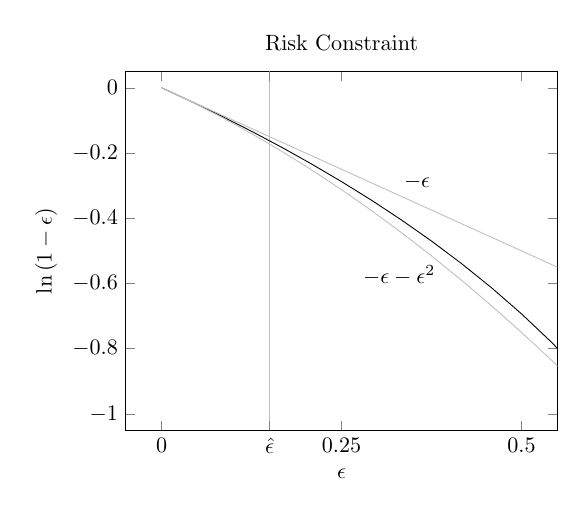
\begin{tikzpicture}[scale=.8]
\begin{axis}[ title=Risk Constraint,xlabel=$\epsilon$,ylabel=$\ln \left( 1-\epsilon \right)$,
  xmin=-.05,xmax=.55,
  ymin=-1.05,ymax=.05,
  xtick={0,.25,.5},
  	extra x ticks={.15},
	extra x tick style={grid=major},
	extra x tick labels={$\hat{\epsilon}$}
]
 \addplot[domain=0:.9999] { ln(1-x) };
 \addplot[domain=0:1,lightgray] {-x};
 \addplot[domain=0:1,lightgray] {-x - x^2};
  \node at (axis cs: .355,-.29) { $-\epsilon$};
  \node at (axis cs: .33,-.575) { $-\epsilon-\epsilon^2$};
\end{axis}
\end{tikzpicture}

\end{center}
\caption{Line risk substitution for individual branches and possible approximations}\label{fig:linerisksub}
\end{figure}




\subsection{System Risk for Multivariate Gaussian Branch Flows}
Now we combine the uncertainty in the effective capacity $\Xi$ with the uncertainty in generation and demand $\bD$.  We assume that the uncertainty spaces $\Xi$ and $\bD$ are orthogonal to each other.  This may not be the case, due to geographically correlated weather which can affect both the effective capacity distribution and the random generation and demand.  Applying the line risk function \Cref{pwl_risk} to the system risk measure \Cref{nofail} and taking the expectation over the random injection space $\bD$, we have
\begin{align}\label{nofailuncertainty}
  \E{\bD}{h(\ry)}  &= \E{\bD}{P_\Xi \left[ \mbox{no lines fail} | \mbox{line flows } \ry\right]}\\
  &= \E{\bD}{ \prod_{e \in \cE} (1 - g_e(\hry_e) )}
\end{align}
since $ 1- g_e(\ry_e) = \bP{\Xi}{\text{Line }e\text{ succeeds} | \ry_e} $ and multiplying over all lines to find the probability that no line fails. The function \Cref{nofailuncertainty} can be approximated by using a linearization of $h(\ry)$.  Let $r$ be the expectated value of the probability that one or more lines fail (the complement of $\E{\bD}{h(\ry)}$). Then, we have
\begin{align*}\label{linear}
r &= \E{\bD}{1 - h(\ry)}  \\
 &= 1 - \E{\bD}{\prod_{e \in \cE}\left( 1 - g_e(\hry_e)\right) } \\
  &= 1 - \E{\bD}{ 1 - \sum_e g_e(\ry_e) + \sum_{e_1,e_2|e_1\neq e_2} g_{e_1} (\ry_{e_1}) g_{e_2}(\ry_{e_2}) - \sum_{e_1,e_2,e_3|e_1\neq e_2 \neq e_3} g_{e_1} (\ry_{e_1}) g_{e_2}(\ry_{e_2}) g_{e_3} (\ry_{e_3}) + \cdots } \\
  & \approx 1 - \E{\bD}{ 1 - \sum_{e} g_e(\ry_e) + \frac{1}{2} \sum_{e_1,e_2|e_1\neq e_2} g_{e_1} (\ry_{e_1}) g_{e_2}(\ry_{e_2}) - \cdots } \\
 &\approx \sum_{e \in \cE} \E{\bD}{g_e(\hry_e)}
\end{align*}
where the approximation derived above comes from taking a Taylor expansions of $h(\cdot)$ at $y=0$ and second order and higher terms.  This approximation is good for small risk values of $h(y)$.
%It is important to note that the linear approximation underestimates system risk and the quadratic approximation overestimates risk for small risk $h(y)$. The risk can also be bounded using the Bonferroni Inequalities, which is a generalization of Boole's Inequality, or the union bound. 
The system risk contributed by line $e$ is integrated over the space $\bD$, which is orthogonal to effective capacity, or likelihood of failure due to loading, $\Xi$.  This system risk measure $r$ captures the endogenous system risk of line failures due to loading under uncertainty in branch flows.

% -----  Picture ----- Gaussian PDF and line failure function ---------------------------------%
\begin{figure}
 \centering                    
  \begin{subfigure}[b]{0.4\textwidth}
   \includegraphics{\mypathjcc/fig-pdfflow}   
   \caption{Probability density of power flow}
  \end{subfigure}
  \begin{subfigure}[b]{.4\textwidth}
    \includegraphics{\mypathjcc/fig-linefail}
    \caption{Line failure density function}
  \end{subfigure}
  \caption{Random Power Flows and the Failure Density Function}
\end{figure}


% -------------------- Linearization for Small Epsilon ENDNOTE -------------------
%To find the linearization for small $t$, the taylor expansion $f(t)=f(t) + \grad f (a)(t-a) +...$ around $a=0$ is useful.  Applying the taylor expansion to our risk measure \ref{nofail}, we end with the linear approximation


Let $ z_e = \E{\bD}{g_e(\ry_e)} $ be the individual line risk. We can break $z_e$ into three segments based upon the value of $\ry_e$ in piecewise linear risk  function \Cref{pwl_risk}.  The first segment for $\hry_e \leq L_e$ has $g_e(\ry_e) = 0$. In the second segment, for $L_e \leq \hry_e \leq U_e^c$, $g_e(\ry_e)$takes an expected value of a truncated normal distribution.  In the last segment, $U_e^c \leq \hry_e$, $g_e(\ry_e)$ takes one and $\ry_e$ is in that segment with the probability calculated from the cumulative distribution function (CDF)  of a normal distribution.  That is,
\[ z_e = 0 +  \E{\bD}{ a+b\hry_e | L \leq \hry_e \leq U^c } \bP{\bD}{L\leq \hry_e \leq U^c}  + 1 * \bP{\bD}{ U^c \leq \hry_e } \] 

 The truncation from the critical capacity $U^c$, the level at which the line fails with certainty, is approximately 0 for choices of $\epsilon$ around a few percent.  If the mean flow $\ry_e$ is at the hard limit $U^{\epsilon}$ defined by risk tolarence $\epsilon$, the following point $ (U^c - U^{\epsilon} )/\sigma $ is the corresponding point in a standard normal distribution and $\Phi \left( (U^c - U^{\epsilon} )/\sigma \right)$ is the probability of being above the critical capacity $U^c$.  When solving this problem, the assumption that $\bP{\bD}{ U^c \leq \hry_e } \approx 0 $ can be checked numerically.  Then, we have
\[ z_e \approx \E{\bD}{ a+b\hry_e | L \leq \hry_e } \bP{\bD}{L\leq \hry_e} \]
The branch flows are truncated Gaussian, which have known mean and variances. Truncated Gaussian's expectation and tail probability are
\[  \E{\bD}{ \hry_e | L \leq \hry_e } = \mu^y_e + \frac{\phi( \alpha_L )}{ 1- \Phi(\alpha_L)} \sigma^y_e \]
\[ \bP{\bD}{ L \leq \hry_e } = 1 - \Phi(\alpha_L) \]
where $\alpha_L = \frac{L - \mu^y_e}{\sigma^y_e}$, the PDF $\phi(\cdot)$ , and the CDF $\Phi(\cdot)$ are for the standard normal distribution.  The line risk  $\rho(\mu^y_e, \sigma^y_e)$ is a function of the mean $\mu^y_e$  and standard deviation $\sigma^y_e$ of the branch flows, given as
\begin{align}\label{line_risk2}
\rho (\mu^y_e,\sigma^y_e) &= \E{\bD}{ a+b\hry_e | L \leq \hry_e } \bP{\bD}{L\leq \hry_e} \\
&= (a + b \mu^y_e)\left[ 1 - \Phi(\alpha_L) \right]  + b \sigma^y_e \phi(\alpha_L) .
\end{align}
Given the approximation to $z_e$ of the truncation of the tail of the distribution, we have
\begin{equation}
z_e \approx \rho (\mu^y_e,\sigma^y_e)
\end{equation}








%%%%%%%% Section 3
\subsection{Joint Chance Constraint Model}%WITH ARBITRARY SLACK!!
The JCC model departs from traditional power flow models in that it allows for a trade-off between line risk, system risk, and cost. Since the cost and risk are both related to the slack distribution, the model is allowed to vary the slack distribution.  In this section, the full joint chance constraint model follows with a brief explanation of some of the constraints.  The relevant parameters derived from the injection covariance matrix is also given.  Then a cutting plane algorithm is shown to solve the full JCC model.

This convex program is minimizing a quadratic cost function of generation $x_j$ for each generator $j \in \cJ$ as well as the expected cost from its participation in the slack distribution $\beta_j$.  The cost coefficients for generator $j$ are $c_j^2,c_j^1,$ and $c_j^0$.  The incidence matrix $c^g_{ij}$ is 1 if generator $j$ is connected to bus $i$.  The incidence matrix $c^b_{ie}$ is 1 if branch $e$ is from bus $i$ and -1 if branch $e$ is to bus $i$.  The parameter $b_e$ is the susceptance of branch $e$ and $U_e^\epsilon$ is the hard limit on branch flow defined by the given risk level in \Cref{hardlimit}.  Each generator $j$ has a risk level $\epsilon_j$ and an associated $\eta_j$ from \Cref{etaequation}.  The standard deviation of aggregate generation and demand uncertain is $\sD$.  The variable $\pi_e$ represents how the slack distribution affects branch $e$ in repsonse to aggregate changes in generation and demand.  The variable $s_e$ represents the standard deviation of branch flow on branch $e$ and $z_e$ represents the probability that line will fail.  The sum of all branch failure probabilities is constrained to be less than the given risk level $\epsilon$.
\begin{subequations}
\label{jcc_program}
\begin{alignat}{3}
\textbf{JCC:= }\min_{\left(x,\beta;\theta,y,\pi,s,z\right)} && \displaystyle\sum_{j \in \cJ} \left[  c^2_j \left(x_j^2 + \beta_j^2 \sD \right) + c_j^1 x_j + c_j^0 \right]  && \label{jcc_obj}\\
                        &&  \sum_{j \in \cJ} c^g_{ij} x_j - \sum_{j \in \cJ} c^b_{ie} y_e          &=d_i       && \forall i \in \cI \label{jcc_cons}\\ 
                 && y_e - b_e  \sum_{i \in \cI} c^b_{ie} \theta_i          &=0         && \forall e \in \cE \label{jcc_kcl}\\
                 && y_e &\in \left[ -U_e^\epsilon, U^\epsilon_e \right] && \forall e \in \cE \label{jcc_limit}\\
                 && x_j + \beta_j \sigma_\Delta \eta_j &\leq G^{max}_j   && \forall j \in \cJ \label{jcc_gen1} \\
                 && x_j - \beta_j \sigma_\Delta \eta_j &\geq G^{min}_j && \forall j  \in \cJ \label{jcc_gen2}\\ 
                 &&  \sum_{j \in \cJ} \beta_j &=1 && \label{jcc_slack}\\
                 && \pe -  \sum_{j \in \cJ} A_{ej} \beta_j   &=0 &&\forall e \in \cE \label{jcc_pi}\\ 
                 && s^2_e - \pi_e^2 \sD + 2 \pi_e \se      &\geq\see &&\forall e \in \cE \label{jcc_var}\\
                 && z_e - g_e(|y_e|,s_e)  &\geq 0 && \forall e \in \cE \label{jcc_lr}\\
                 &&  \sum_e z_e &\leq \epsilon && \label{jcc_risk}
\end{alignat}
\end{subequations}


The objective \Cref{jcc_obj} for the JCC model is the typical quadratic objective for the OPF model plus a contribution from the slack distribution due to the uncertainty in the random injects.  This objective is the expected cost of meeting the realized demand.  We use individual chance constraints to deal with the uncertainty in load for \Cref{jcc_gen1,jcc_gen2} with $\eta_g = \Phi^{-1}(1-\epsilon_g)$ being its tolerance.  The upper and lower bounds on generator levels $[G^{min},G^{max}]$ are dependent on many things, most importantly the time frame used.  The levels are affected by the status of the generator (on,off,starting up,shutting down),  its ramping rate, and any other physical limits it may have.  

The first equations \Cref{jcc_obj,jcc_cons,jcc_kcl,jcc_slack,jcc_limit} are your typical DC power flow, \Cref{jcc_gen1,jcc_gen2} are chance constraints on generators, and the last set \Cref{jcc_pi,jcc_var,jcc_lr,jcc_risk} describe system risk.  The branch variance \Cref{jcc_var} are a second order cone and the line risk \Cref{jcc_lr} involve the CDF of a normal distribution.  These equations are solved via a cutting plane approach so that the individual subproblems are linear programs.


\subsection{Solution Methodology}\label{solutionmethodology}
Since the risk function is convex, we choose cutting planes to approximate the line risk constraints \Cref{jcc_lr}.  In addition, there were many second order cone constraints (number of lines).  Instead of using these constraints explicitly, they were added through cutting planes as well.  This kept the program to a manageable size and allowed for fast solve times.  

\begin{lemma}
The line risk function \Cref{line_risk2} is convex with respect to $\mu^y_e$ and $\sigma^y_e$
\end{lemma}
\begin{proof}
Starting with the line risk function \Cref{line_risk2}
\begin{equation*}
\rho_e(\mu^y_e,\sigma^y_e) = (a_e + b \mu^y_e)\left[ 1 - \Phi(\alpha_L) \right]  + b \sigma^y_e \phi(\alpha_L) 
\end{equation*}
First, we calculate $\frac{\partial \Phi(\alpha_L)}{\partial \mu^y_e} = - \frac{1}{\sigma^y_e} \phi(\alpha_L)$ and $\frac{\partial \phi(\alpha_L)}{\partial \mu^y_e} =  \frac{1}{\sigma^y_e} \alpha_L \phi(\alpha_L)$ using the chain rule.  Now note that from our piecewise linear function \Cref{pwl_risk}, we have the identity $L = -\frac{a_e}{b_e}$. Then, taking the derivative of $\rho$ with respect to $\mu^y_e$, we get  
\begin{align*}
\frac{\partial \rho_e}{\partial \mu}(\mu^y_e,\sigma^y_e) &= (a_e + b_e \mu^y_e) \frac{1}{\sigma^y_e} \phi(\alpha_L) + b_e \left[ 1 - \Phi(\alpha_L) \right] + b_e \alpha_L \phi(\alpha_L)\\
&= \frac{a_e + b_e \mu^y_e}{\sigma^y_e}\phi(\alpha_L)  + b_e \left[ 1 - \Phi(\alpha_L) \right] +  \frac{b_e L_e - b_e\mu^y_e}{\sigma^y_e}\phi(\alpha_L) \\
&= \frac{a_e + b_e \mu^y_e}{\sigma^y_e}\phi(\alpha_L)  + b_e \left[ 1 - \Phi(\alpha_L) \right] -  \frac{a_e + b_e\mu^y_e}{\sigma^y_e}\phi(\alpha_L)\\
& = b_e\left[ 1 - \Phi(\alpha_L) \right]
\end{align*}
For our derivative with respect to $\sigma^y_e$, we calculate $\frac{\partial \Phi(\alpha_L)}{\partial \sigma^y_e} = - \frac{1}{\sigma^y_e} \alpha_L \phi(\alpha_L)$ and $\frac{\partial \phi(\alpha_L)}{\partial \sigma^y_e} =  \frac{1}{\sigma^y_e} \alpha_L^2 \phi(\alpha_L)$.  Then, taking the derivative of $\rho$ with respect to $\sigma^y_e$, we have
\begin{align*}
\frac{\partial \rho_e}{\partial \sigma}(\mu^y_e,\sigma^y_e) & = (a_e+b_e\mu^y_e)\frac{1}{\sigma^y_e} \alpha_L  \phi(\alpha_L) + b_e \sigma^y_e \frac{1}{\sigma^y_e} \alpha_L^2  \phi(\alpha_L) + b_e \phi(\alpha_L)\\
& = -b_e\frac{L-\mu^y_e}{\sigma^y_e} \alpha_L  \phi(\alpha_L) + b_e \alpha_L^2  \phi(\alpha_L) + b_e \phi(\alpha_L)\\
 & = b_e \phi(\alpha_L) 
\end{align*} 
where the identities $a_e=-b_eL_e$ and $\alpha_L = \frac{L_e-\mu^y_e}{\sigma^y_e}$ were used.

The Hessian is found with the second derivatives and is given by
\begin{equation}
\grad^2 \rho_e(\mu^y_e,\sigma^y_e) = \frac{b_e \phi(\alpha_L)}{\sigma}
\left[ 
\begin{array}{c c}
1 & \alpha_L \\
\alpha_L & \alpha_L^2
\end{array}
\right]
\end{equation}
Then, we note that the determinant is 0 and the diagonal elements are positive so that there is a positive eigenvalue and a zero eigenvalue, thus the line risk is convex with respect to $\mu^y_e, \sigma^y_e$.  Since system risk is approximated by the sum of line risks, this system risk measure is convex. \qed
\end{proof}

 Since the inequality \Cref{jcc_lr} is convex, we can solve this using a cutting plane approach to describe the line risk in terms of the mean branch flow $y_e$ and the standard deviation of branch flow $s_e$.  While there are infinitely many cuts, this program can be solved for a given error tolerance with a finite, and typically small, set of cuts.
\begin{subequations}
\label{line_risk_cuts}
\begin{align}
z_e \geq \rho_e(\hye,\hse) &+ \frac{\partial \rho}{\partial y_e}(\hye,\hse) \left(y_e - \hye \right) 
+ \frac{\partial \rho}{\partial s_e}(\hye,\hse) \left(s_e - \hse \right) \\
\rho_e(y_e,s_e) &= (a_e + b_e y_e)\left[ 1 - \Phi(\alpha_L) \right]  + b_e s_e \phi(\alpha_L)  \\
 \frac{\partial}{\partial y_e}\rho_e(y_e,s_e) &= b_e\left[ 1 - \Phi(\alpha_L) \right]\\
\frac{\partial}{\partial s_e}\rho_e(y_e,s_e) &= b_e \phi(\alpha_L) 
\end{align}
\end{subequations}

The standard deviation of branch flow can be formulated as a second order cone with respect to the slack distribution variables.  While this could be solved with a commercial solver, we proceed with a cutting plane approach to speed up solve times.  As the solution approach is already iteratively improving system risk, it adds only a small amount of work to add these cuts as well and reduces the subproblem to a linear program.  The inequallities required to approximate the nonlinear constraints \Cref{jcc_var} are:
\begin{subequations}
\label{branch_var_cuts}
\begin{align}
s_e \geq \fehb &+ \sum_{j \in \cJ} \pfehb \left( \beta_j - \hat{\beta_j} \right)\\
  \feb &= \sqrt{\pe^2 \sD - 2 \pe \se  + \see }\\
  \pfeb &= \frac{A_{ej} \left( \pe \sD - \se \right)}{\sqrt{\pe^2 \sD - 2 \pe \se  + \see }}
\end{align}
\end{subequations}




\subsubsection*{Cutting Plane Algorithm}
Now, we can describe the cutting plane algorithm for JCC at a high level. Algorithm \ref{jcc_alg} is pseudo code for the implementation.  The main subproblem the algorithm solves is the standard DC power flow, which is defined by \Cref{jcc_obj,jcc_cons,jcc_kcl,jcc_slack,jcc_limit} .  After solving, the generator injects $x$, slack distribution $\beta$, and branch flows $y$ are used to calculate risk information about the dispatch point.  To get the risk information, the branch standard deviations $s$ need to be calculated.  With the mean flow $y$ and standard deviation $s$, the line risk $z$ can be calculated.  The sum of line risk is the system risk $r$.  If $r$ is less than the required system risk $\epsilon$, the problem is solved.  Otherwise, the algorithm adds cuts for all lines with a positive risk $z$.  The cuts describe how risk $z$ is related to branch flows $y$,standard deviation $s$ and how $s$ is related to $\beta$.  Then the power flow subproblem is solved with the addition of the cuts and this repeats until it is infeasible or the risk constraint is satisfied.
\begin{algorithm}
\caption[Cutting plane algorithm for joint chance constraint model]{This cutting plane algorithm solves JCC \Cref{jcc_program} via linear programs and cutting planes}\label{jcc_alg}
\begin{algorithmic}
\Procedure{JCC}{d,$\Sigma^m$,$\epsilon$,$\epsilon_g$,L,p}
\State $L \gets \emptyset$  (Set of Lines with potential risk)
\State $S \gets \emptyset$  (Set of Cuts)
\State $r \gets 0$ (Risk)
\BState \emph{solve}:
\State $(\hat{x},\hat{\beta},\hat{y}) \gets $Solve DC Power Flow, \Cref{jcc_obj,jcc_cons,jcc_kcl,jcc_slack,jcc_limit,jcc_gen1,jcc_gen2}, with cuts $S$, risk $r\leq\epsilon$
\If {Infeasible} \Return Problem Infeasible 
\EndIf
\State Calculate $\hat{s},\hat{z},\hat{r}$ using $(\hat{x},\hat{\beta},\hat{y})$ and \Cref{branch_cov,line_risk}
\If {$\hat{r} \leq \epsilon + tol$} \Return Optimal $(\hat{x},\hat{\beta},\hat{y},\hat{s},\hat{z},\hat{r})$
\EndIf
\For{$\forall e$}
\If {$\hat{z_e} \geq tol$}
    \If {$e \notin L$}
            \State $L \gets \left\{L,e\right\}$
            \State Initialize $s_e,z_e$
            \State $r \gets r + z_e$
    \EndIf            
    \State $S \gets$ line risk cuts \Cref{line_risk_cuts} for $z_e,y_e,s_e$ dependent on $\hat{z}_e,\hat{y}_e,\hat{s}_e$
    \State $S \gets$ branch variance cuts \Cref{branch_var_cuts} for $s_e,\beta_e$ dependent on $\hat{s}_e,\hat{\beta}_e$
\EndIf
\EndFor
\State \textbf{goto} \emph{solve}
\EndProcedure
\end{algorithmic}
\end{algorithm}





%%%%%%%% Section 5
\section{Computational Experiments}\label{computationalresults}
This section explains the computation setup, the test cases, the experiments performed, and the intuition to gain from the comparison of OPF, CC, and JCC models.
\subsection{Implementation of the JCC Model}
All of the experiments are run on a laptop with an Intel i7-3537U processor with 2 cores,4 threads at 2.00GHz.  The laptop has 8GB of memory, but even with the large instances (2383 buses), memory is not an issue.  The laptop is running Linux Mint Petra 16.  The OPF, CC, and JCC models are all solved within a C++ program.  The program uses Armadillo\cite{armadillo} for linear algebra computation and Concert and CPLEX to solve the linear programs.  CPLEX is run with default settings and the dual simplex algorithm is used to solve the linear programs (quadratic objective for the 30 bus test case).  All time comparisons are using the same system environment with a fixed clocked speed and few programs in background.  The primary DC OPF solver in the C++ program has been developed to output nearly identical results to Matpower\cite{matpower}.
\subsection{Single Instance}
The test cases are all taken from Matpower test cases.  The two test cases used are the 30 bus test case as well as the 2383wp test case.  The small test case is used to show properties of the different dispatch points and the cost-risk frontier.  The large test case is used for time trials as well as a cost-risk scatter plot.  

\subsubsection*{30 Bus Case}
This case from Matpower has 30 buses, 41 branches, and 6 generators.  The branches have a single capacity rating and in the given demand scenario, none of the line capacity  constraints are active.  A capacity factor $M$ is used to uniformly scale the branch capacities.  All of the generators are active and have quadratic cost functions.  Ramping constraints for generators are not considered and the generators are allowed to take any value in its given range.  In addition, all generators are allowed to participate in the slack distribution.  Each bus with a demand is considered random, with mean equal to the demand.  For this example, the injections are independent of each other but this need not be the case.  The variance of each injection is equal to 5\% of the demand at the node times a budget factor $B$ used to tune the model uncertainty level.

\begin{table}
\centering
\begin{tabular}{ |c| c c c |}
\hline
& OPF & CC & JCC \\
\hline
\hline
Cost & 567.1 & 574.0 & 565.2\\
$r$ & 0.0171 & 0.0179 & 0.0080\\
\hline
\end{tabular}
\caption{Cost and risk results for OPF,CC, and JCC models on the small test case}\label{solve_results}
\end{table}

\begin{table}
\centering
\small
\begin{tabular}{| c| c |c c c c c c |}
\hline
 &     &   &   &  Generator & & & \\
 & Mod & 1 & 2 & 3 & 4 & 5 & 6 \\
\hline
\hline
$\left[ g_{min}, g_{max} \right]$& & [0,80]&[0,80] &[0,50] &[0,55] &[0,30] &[0,40]  \\
$\left\{ c_2, c_1 \right\}$ && $\left\{0.02,2\right\}$  &$\left\{0.0175,1.75\right\}$ &$\left\{0.0625,1\right\}$ &$\left\{0.00834,3.25\right\}$ &$\left\{0.025,3\right\}$ &$\left\{0.025,3\right\}$  \\
\hline
\hline
$x_g$ &OPF& 39.7  &  52.3  &  24.2  &  35.7  &  19  &  18.3   \\
$x_g$ &CC& 35.9  &  47.9  &  25.7  &  37.2  &  19.3  &  23.1    \\
$x_g$ &JCC& 41.9  &  55.0  &  23.2  &  34.0  &  18.6  &  16.5    \\
\hline
$\beta_g$ &OPF& 0.1548  &  0.1769  &  0.0495  &  0.3712  &  0.1238  &  0.1238    \\
$\beta_g$ &CC& 0  &  0  &  0.4411  &  0.2986  &  0  &  0.2602   \\
$\beta_g$ &JCC& 0.2456  &  0.2795  &  0.0846  &  0.0646  &  0.0597  &  0.2659   \\
\hline
\end{tabular}
\caption{Generator results using OPF, CC, and JCC models on the small test case.}\label{solve_one}
\end{table}

The first example has risk parameters $L=0.9$, that is a line  begins taking on risk after it is at 90\% of its rated capacity.  In the risk function, we set the parameter $p_e=0.005$ for all branches $e$, which means that if flow is at nominal capacity, the line has a $0.5\%$ chance of failing.  The line capacities are scaled by $M=0.745$. The system risk constraint is $\epsilon=0.008$, that is we would like to enforce that the risk of one or more lines failing is less than or equal to  $0.8\%$.  The chance constrained version of OPF is defined by $\eta_L=0.05$, that is the line capacities can not be violated more than $5\%$ of the time.  Finally, the variance of the injects is scaled by $B=0.025$ so that the standard deviation of aggregate demand is $0.6$, a small fraction of the total demand, $189.2$, of this instance.  These values were chosen to get the objective values close and highlight how the uncertainty in generation and demand affect the models differently. The solution values for generation and slack distribution $(x,b)$ are tabulated in \Cref{solve_results,solve_one}.  Increasing $B$ to $0.25$ by 10 fold led to the standard deviation of aggregate demand to be $1.345$, around 1\% of total load.  The cost of OPF and JCC had negligible change, whereas CC cost increased to \$597, an increase of \$30 or an increase of 5\% over the OPF solution. When the OPF model has transmission congestion, the cost of the CC model is highly sensitive to the uncertainty in demand  and  often infeasible solutions.



The CC model is always more conservative than the OPF model as it tightens the line constraints.  This means that the CC version is always at least as expensive as the OPF model.  In this case, the total cost rose by \$7 (to \$574, or a 1.2 \% increase) to ensure the line constraints were met probabilistically (95\% of the time).  The JCC model was able to lower the cost because it removed the branch capacity constraints (or increased them by 6\% to match the system risk level).  In addition, JCC knows and constrains the system risk measure so that it is able to find a cheaper point with a system risk level half that of the OPF and CC models.



Another important note is that the slack would like to be distributed as much as possible to reduce cost.  This can be seen from the objective \Cref{jcc_obj} due to the squared beta term and the OPF results show it spreading when there is no chance constraints for lines or system risk constraints.  The CC model slightly changes its generator position as well as removing 3 generators from the slack distribution.  It is removing generators which has an effect on the probabilistically constrained transmission lines in order to ensure that the constraints are met $95\%$ of the time.  The JCC model has moved in almost exactly the opposite direction and has kept a distributed slack (as seen in \Cref{solve_one}).




\subsubsection*{Cost-Risk Frontier}
  \begin{figure} % redo with new operating models
\centering
\includegraphics{\mypathjcc/fig-costrisk}
\caption{Reliability frontier for the small test case}\label{costriskfront}
\end{figure}
%pow case/30.db  .775 1.1 1 .00195 .4 .00275 .5 .9 .005 .4 1000 2> cost-risk.dat
%m0   m1          mg   eps epsN     pL pG     L  p  B    T
%0.775            1.1  1   0.00195  0.4       0.00275    0.5     0.9     0.005   0.4     1000
Now we use this same example case to draw a cost-risk frontier.  An efficient operating point would be at that boundary of the feasible points, that is, neither cost nor risk can be improved without a loss to the other.  Since neither the OPF or CC model constrains our risk measure, it would be unlikely for them to be on the boundary.  In \Cref{costriskfront} we see that this is the case.  The OPF model is in the interior and is equivalent to the CC model when $\eta_l=.5$.  Since the branch flows are Gaussian, if the mean flow is at its threshold, it has a 50\% chance of being over its threshold.  As $\eta_l$ is reduced, the CC line is drawn and is stopped once the system becomes infeasible.  The JCC line is started by finding the point when the system risk level is not constrained, for this case $r=.01$.  As $r$ is decreased, the system risk becomes constrained and the cost begins to rise as the risk level is reduced and the line stops when the system becomes infeasible.  We used parameters $M=0.775$ for line capacity scaling and $B=0.4$ with standard deviation of aggregate load being around $1\%$ of total demand.  The left plot uses $L=.9$ for calculating the system risk measure whereas the right plot uses $L=.99$ to calculate the system risk measure.  In practice, it was found that as $L$ gets closer to 1, the model behaves more like the CC model.


It is important to note that the cost-risk frontier is entirely dependent on how system risk is measured.  In our case, we use a piecewise linear failure density function with parameters $L$ and $p$.  As $L$ and $p$ are varied, the shape of these frontiers changes.  Holding $p$ fixed and increasing $L$ towards 1, the CC model, while still on the interior of the frontier, does a better job of reducing system risk.  With $L$ around .98, the CC and the JCC behave similarly.  Both programs try to reduce the flow of lines that are at their capacity, with the exception that JCC allows a small number (typically one), of flow on these lines to increase.  More discussion on this behavior is given in the sensitivity analysis \Cref{senseanal}.


\subsubsection*{2383wp Bus Case}
This case from Matpower has 2383 buses, 2896 branches, and 327 generators.  The case is similar to the small case in many respects, such as only a single line rating capacity being given.  The generators have the biggest difference in that there are many which are nearly fixed and have no cost.  The larger flexible generators are only given a linear cost so that there is no quadratic objective.  The covariance matrix is developed the same as in the small case, i.e. with no covariance in random injects and the variance depending on the total demand of each node

Similar to the 30 bus case, we created a random instance using parameters $M=1.03, \epsilon=0.03, \eta_L=0.05, L=0.85, p=0.005$, and $B=1$ and recording the standard cost and risk information as well as solve time.  The case was repeated 10 times and the mean time is reported in \Cref{solve_time}.  CC and JCC take a similar amount of time, the majority of the work at each step being the calculation of the branch covariance matrix.  The total time is largely dependent on how many iterations the algorithms take, which is typically around 5 or 7 until convergence. 

In addition, we solved 100 instances with random demand and the same covariance matrix to show the speed-up you can achieve with repeated solves.  By having the same covariance matrix, all of the cuts for previous solves are still valid.  So, in addition to using a warm start on the LP, after the first few solves the algorithm typically needs no additional cuts.  In practice, this could mean that the important lines and scenarios from the risk perspective are known before hand and cuts are added based on the assumed covariance matrix.  Instead of taking up to 5 to 7 iterations, it may solve in only one and perform a simple check to ensure that any lines not included in the analysis are not violated.  The last row in \Cref{solve_time} shows that the solve time was reduced from on around 8 seconds to around 2 seconds.

\begin{table}
\centering
\begin{tabular}{| c| c c c| }
\hline
Time ($\eta_L,\epsilon$) & OPF & CC & JCC \\
\hline
\hline
Time (0.05,0.03)& 0.37  & 8.7 & 7.5 \\
%Time (0.10,0.05)& 0.37 & 8.6  & 7.4  \\
Time (0.20,0.07)& 0.37  & 8.4 & 8.0 \\
%Time (0.30,0.10)& 0.37  & 8.4 & 7.6 \\
Time (0.40,0.20)& 0.37  & 8.3 & 6.1 \\
%Time (0.45,0.30)& 0.37  & 8.3 & 6.1 \\
Time (0.48,0.30)& 0.37  & 7.7 & 6.1 \\
\hline
\hline
Avg Time (100 trials)& 0.34  & 2.2 & 2.3 \\
\hline
\end{tabular}
\caption{Time comparison, in seconds, for OPF,CC, and JCC on the large test instances.}\label{solve_time}
\end{table}

\subsubsection*{Line Threshold Comparison}
Here we explore what the JCC model is doing to lower its cost or risk compared to the traditional models.  For this experiment, the parameters are as follows, $M=1.03, \epsilon=0.015, \eta_L=0.05, L=0.95, p=0.005$, and $B=1$.  Solving this program, we see that the majority of the lines are less than 50\% utilized.  There are a small number of lines that are at or near their nominal capacity.


\begin{figure}
\centering
\begin{subfigure}[b]{0.4\textwidth}
\includegraphics{\mypathjcc/fig-normflow}
\caption{All lines that have mean flow (in OPF) above 95\% of nominal capacity}\label{solve_shadow}
\end{subfigure}
\hspace{15px}
\begin{subfigure}[b]{0.4\textwidth}
\centering
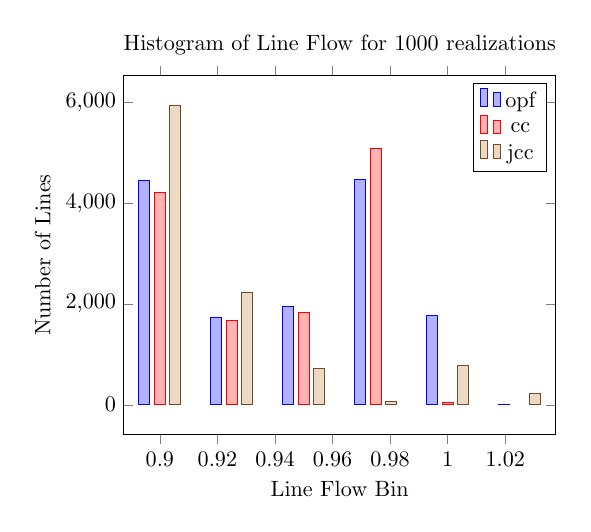
\begin{tikzpicture}[scale=.8]
\begin{axis}[title=Histogram of Line Flow for 1000 realizations, 
    xlabel=Line Flow Bin, 
    ylabel=Number of Lines,
x tick label style={
/pgf/number format/1000 sep=},
  ybar, bar width=5pt ,
  enlargelimits=0.1]
\addplot coordinates { ( 0.9,4450)  ( 0.925,1729)  ( 0.95,1949)  ( 0.975,4471)  ( 1,1770)  ( 1.025,3) };
\addplot coordinates { ( 0.9,4219)  ( 0.925,1678)  ( 0.95,1834)  ( 0.975,5077)  ( 1,53) };
\addplot coordinates { ( 0.9,5931)  ( 0.925,2218)  ( 0.95,711)  ( 0.975,70)  ( 1,784)  ( 1.025,221) };
\legend{opf,cc,jcc}
\end{axis}
\end{tikzpicture}

\caption{Histogram to compare high flow lines of OPF,CC, and JCC}\label{histogram}
\end{subfigure}
\end{figure}

Now, we look at the trade-off that the JCC model is able to make due to it increasing the nominal line limit by 10\% to match the given system risk level.  In  \Cref{solve_shadow}, 8 lines are shown, which are the lines above 95\% of their nominal capacity in the OPF model.  The mean line flows are plotted as well as the standard deviation.   There are 8 lines above 95\% of their capacity in the OPF model, indexed as lines 23,291,320,1380,1381,1815,2108, and 2109. In the OPF model, there are 3 lines at the nominal capacity.  Line 23 (index 1 in figure) has a dual price of 872, line 291 (index 2) has a dual price of 32, and line 2108 (index 8) has a dual price of 294.  Ideally, line 23 constraint should be relaxed due to the higher shadow price and perhaps other lines further constrained so that the system risk level is not increased. However, in the CC model, these constraints are tightened further to ensure that these thresholds are met at least 95\% of the time.  The JCC model on the other hand relaxes these constraints and imposes a system risk constraint instead.  The final solution for the JCC model has line 23 exceed its threshold with certainty but is rewarded with savings related to the high shadow price.  On the other hand, other lines with positive line risk are be restricted to ensure the system risk levels are met.

To give another perspective, the line flows were sampled and binned to create a histogram of line flows to show the trade-off between models.  For the JCC model, the line risk parameter $L$ was chosen to be 0.9.  The results can be seen in \Cref{histogram}.  We can see that the normalized line flows pile up in bin 0.975 for the CC model, and there are a number of lines in OPF that are in bin $1-1.025$, thus exceeding their capacity a significant amount of the time.  The JCC also has a line that exceeds its capacity, almost with certainty.  However, the JCC has far fewer lines that are at or near their capacity.



The primary strength of the CC model is to meet the line threshold constraints probabilistically when the demands are not known with certainty.  Let's look at how well it does from the system perspective, that is the expected number of lines to be over their nominal capacity, shown in \Cref{solve_risk}.  First we note the costs, both CC and JCC are around 5\% higher and in return for the higher cost, have better risk characteristics.  In the standard OPF model, the expected number of lines over their threshold is 20 times that of the CC model.  The JCC halves the CC model for roughly the same cost.  The CC model directly constraints these probabilities, but does so on the individual line level.  By having a system constraint, the JCC model is better suited to optimize risk characteristics related to system level transmission utilization.


\begin{table}
\centering

 \begin{tabular}{ |c| c c c |}
\hline
& OPF & CC .01 & JCC .98 \\
\hline
\hline
Cost & 565.2 & 590.2 & 589.6 \\
$r$ & 0.00504 & 0.00150 & 0.00031 \\
\hline
$Ex$ & 0.3875 & 0.0225 & 0.0125 \\
\hline
\end{tabular}
\caption{Risk comparison for OPF,CC, and JCC on the small test instance.}\label{solve_risk}
\end{table}


\subsection{Sensitivity Analysis}\label{senseanal}
Now, we want to look at the sensitivity of the JCC model to its input parameters and demand uncertainty.  First we look at how the risk of the different dispatch points from the OPF, CC, and JCC models respond to changes in the failure density function parameters $L$ and $p$.  To this end, we solved the OPF, CC ($\eta_L=.01$), and JCC ($\epsilon=0.0003$, $L=.98$).  These three dispatch points are used to find the risk of the branch flows for varying risk parameters $L,p$. The cost of the dispatch points are shown in \Cref{tabsense} and the sensitivity analysis is shown in \Cref{figsense}. This figure shows that for the given JCC solution, the system risk stays under that of the CC model.  The OPF model has a lower cost so it is reasonable that the risk is much higher.  Even when changing to other polynomial risk functions, such as $x^2,x^3,$ and $x^4$, the JCC model performed better in terms of this alternative risk function than the OPF and CC models.  These parameters are very difficult to estimate in the real world and as such it is very important that our model has shown to be robust to changing both the parameters in the piecewise linear model as well as testing against different polynomial models for failure density functions.  This sensitivity analysis shows that while our parameters may be off, this model still does well for the assumptions that at some point, lines begin to take on additional risk due to congestion and that risk is monotonically increasing.

\begin{table}
\centering
 \begin{tabular}{ |c| c c c |}
\hline
& OPF & CC & JCC \\
\hline
\hline
Cost & 567.1 & 574.0 & 572.2\\
\hline
\end{tabular}
\caption{Table of cost for the three dispatch points used in the sensitivity analysis}\label{tabsense}
\end{table}


\begin{figure}
\centering
\includegraphics{\mypathjcc/fig-sensitivity}
\caption[A comparison of the three dispatch points for varying risk function parameters]{A comparison of the three dispatch points created by fixing $p$ and varying $L$}\label{figsense}
\end{figure}






%%%%%%%% Section 6
\section{Conclusion}


The primary strength of the JCC model is the addition of a system risk constraint and the relaxation of line thresholds. Line thresholds are hard constraints that subject the system to price spikes.  The hard line constraints are somewhat arbitrary as the line does not fail when it is exceeded by a small amount.  Instead, an economic trade-off should be made between individual lines to ensure the system risk is constrained at an adequate level.  The system risk measure allows for direct comparison of different dispatch points with respect to risk.

The JCC model is computationally efficient in its full form.  It allows for creation of a cost-risk frontier that finds dispatch points that are better in both terms of risk and cost.  Under uncertainty, this model should be compared against the CC model, which is a probabilistic interpretation of line thresholds.   In the computational section, we saw the extremely high sensitivity of cost to uncertainty in load when the transmission system is congested.  In both of these models, the variable slack distribution plays a small direct role in cost through the objective, however also plays a role in ensuring the line and system risk constraints are met (and a larger indirect cost contribution).  These system risk constraints capture the risk of a heavily loaded transmission system that the traditional OPF and CC miss that is related to cascading power failure risk in literature.
  
%Combining the system risk measure and random power injects for the joint chance constrained model accounts for many things the traditional OPF model misses.  This model gives prices for system response to aggregated random injects, which is regulation and reserve support for different time periods.  Instead of having an ancillary service model which separates this, the JCC model directly accounts for it.  This allows for valuing random injects, which is important going forward as the grid integrates more uncertain generation (wind turbines) and demand (electric vehicles).


%There are many avenues to improve and extend this model.  Effective capacities are related to environmental conditions, such as high wind,  and as such, are often correlated.  During high wind periods, there is increased wind generation as well as increased effective capacities, which means that when the turbines are producing more energy, the nearby transmission lines are also capable of carrying more energy.  

%Finally, the random injects need to be priced and accounted for.  Random injects add stress to the grid which needs to be secured through ancillary markets such as operating reserves and regulation.
